% Add figures
% Add indexes and documentaion
% Still true?
\subsection{Database Design}
We use a database on our server, to keep track of who owns which files, who has access and who made what changes to them.\\
Our relational database contains eight tables:\\
\textbf{User} describes a user. Email is used as primary key\\
\textbf{File} describes a file on the server. We use serverpath to describe the path to the folder where the file is located, and name as file name. We don't keep track of folders. By specifying the path to the folder of the file, describing folders become unnecessary. Only downside is that we are unable to handle empty folders as an empty folder is not described by any files. The File table can also hold a Project ID, if the file is a part of a project.\\
\textbf{FileMetaData} holds meta date for a file such as resolution for pictures. Has a reference to MetaDataType and holds a value.\\
\textbf{MetaDataType} describes different kinds of meta data. One type may be used by vast amount of files.\\
\textbf{FileInstance} is a relation between User and File. This describes the local path for a specific user, which allows different users to store their copy of a file, in different locations.\\
\textbf{Change} is used to keep track of who changed what in which file at what time.\\
\textbf{Project} holds the title of the project.\\
\textbf{ProjectHasUser} keeps track of which projects a user has.\\
\begin{figure}[h]
  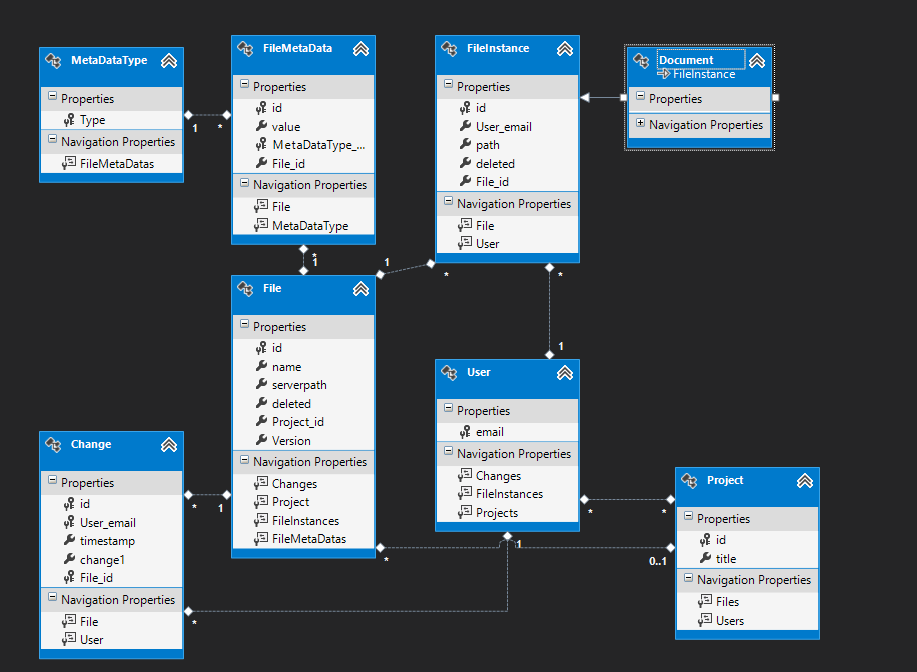
\includegraphics[width=\textwidth,natwidth=793,natheight=635]{illustrations/entitymodel.png}
  \caption{Entity Model}
  \label{entitymodel}
\end{figure}